\documentclass[a4paper, 14pt]{extarticle}

% Поля
%--------------------------------------
\usepackage{geometry}
\geometry{a4paper,tmargin=2cm,bmargin=2cm,lmargin=3cm,rmargin=1cm}
%--------------------------------------


%Russian-specific packages
%--------------------------------------
\usepackage[T2A]{fontenc}
\usepackage[utf8]{inputenc} 
\usepackage[english, main=russian]{babel}
%--------------------------------------

\usepackage{textcomp}

% Красная строка
%--------------------------------------
\usepackage{indentfirst}               
%--------------------------------------             


%Graphics
%--------------------------------------
\usepackage{graphicx}
\graphicspath{ {./images/} }
\usepackage{wrapfig}
%--------------------------------------

% Полуторный интервал
%--------------------------------------
\linespread{1.3}                    
%--------------------------------------

%Выравнивание и переносы
%--------------------------------------
% Избавляемся от переполнений
\sloppy
% Запрещаем разрыв страницы после первой строки абзаца
\clubpenalty=10000
% Запрещаем разрыв страницы после последней строки абзаца
\widowpenalty=10000
%--------------------------------------

%Списки
\usepackage{enumitem}

%Подписи
\usepackage{caption} 

%Гиперссылки
\usepackage{hyperref}

\hypersetup {
	unicode=true
}

%Рисунки
%--------------------------------------
\DeclareCaptionLabelSeparator*{emdash}{~--- }
\captionsetup[figure]{labelsep=emdash,font=onehalfspacing,position=bottom}
%--------------------------------------

\usepackage{tempora}

%Листинги
%--------------------------------------
\usepackage{listings}
\lstset{
  basicstyle=\ttfamily\footnotesize, 
  %basicstyle=\footnotesize\AnkaCoder,        % the size of the fonts that are used for the code
  breakatwhitespace=false,         % sets if automatic breaks shoulbd only happen at whitespace
  breaklines=true,                 % sets automatic line breaking
  captionpos=t,                    % sets the caption-position to bottom
  inputencoding=utf8,
  frame=single,                    % adds a frame around the code
  keepspaces=true,                 % keeps spaces in text, useful for keeping indentation of code (possibly needs columns=flexible)
  keywordstyle=\bf,       % keyword style
  numbers=left,                    % where to put the line-numbers; possible values are (none, left, right)
  numbersep=5pt,                   % how far the line-numbers are from the code
  xleftmargin=25pt,
  xrightmargin=25pt,
  showspaces=false,                % show spaces everywhere adding particular underscores; it overrides 'showstringspaces'
  showstringspaces=false,          % underline spaces within strings only
  showtabs=false,                  % show tabs within strings adding particular underscores
  stepnumber=1,                    % the step between two line-numbers. If it's 1, each line will be numbered
  tabsize=2,                       % sets default tabsize to 8 spaces
  title=\lstname                   % show the filename of files included with \lstinputlisting; also try caption instead of title
}
%--------------------------------------

%%% Математические пакеты %%%
%--------------------------------------
\usepackage{amsthm,amsfonts,amsmath,amssymb,amscd}  % Математические дополнения от AMS
\usepackage{mathtools}                              % Добавляет окружение multlined
\usepackage[perpage]{footmisc}
%--------------------------------------

%--------------------------------------
%			НАЧАЛО ДОКУМЕНТА
%--------------------------------------

\begin{document}

%--------------------------------------
%			ТИТУЛЬНЫЙ ЛИСТ
%--------------------------------------
\begin{titlepage}
\thispagestyle{empty}
\newpage


%Шапка титульного листа
%--------------------------------------
\vspace*{-60pt}
\hspace{-65pt}
\begin{minipage}{0.3\textwidth}
\hspace*{-20pt}\centering

\includegraphics[width=\textwidth]{emblem}
\end{minipage}
\begin{minipage}{0.67\textwidth}\small \textbf{
\vspace*{-0.7ex}
\hspace*{-6pt}\centerline{Министерство науки и высшего образования Российской Федерации}
\vspace*{-0.7ex}
\centerline{Федеральное государственное бюджетное образовательное учреждение }
\vspace*{-0.7ex}
\centerline{высшего образования}
\vspace*{-0.7ex}
\centerline{<<Московский государственный технический университет}
\vspace*{-0.7ex}
\centerline{имени Н.Э. Баумана}
\vspace*{-0.7ex}
\centerline{(национальный исследовательский университет)>>}
\vspace*{-0.7ex}
\centerline{(МГТУ им. Н.Э. Баумана)}}
\end{minipage}
%--------------------------------------

%Полосы
%--------------------------------------
\vspace{-25pt}
\hspace{-35pt}\rule{\textwidth}{2.3pt}

\vspace*{-20.3pt}
\hspace{-35pt}\rule{\textwidth}{0.4pt}
%--------------------------------------

\vspace{1.5ex}
\hspace{-35pt} \noindent \small ФАКУЛЬТЕТ\hspace{80pt} <<Информатика и системы управления>>

\vspace*{-16pt}
\hspace{47pt}\rule{0.83\textwidth}{0.4pt}

\vspace{0.5ex}
\hspace{-35pt} \noindent \small КАФЕДРА\hspace{50pt} <<Теоретическая информатика и компьютерные технологии>>

\vspace*{-16pt}
\hspace{30pt}\rule{0.866\textwidth}{0.4pt}
  
\vspace{11em}

\begin{center}
\Large {\bf Лабораторная работа № 9} \\ 
\large {\bf по курсу <<Языки и методы программирования>>} \\
\large <<Перегрузка операций>> 
\end{center}\normalsize

\vspace{8em}


\begin{flushright}
  {Студент группы ИУ9-21Б Горбунов А. Д. \hspace*{15pt}\\ 
  \vspace{2ex}
  Преподаватель Посевин Д. П.\hspace*{15pt}}
\end{flushright}

\bigskip

\vfill
 

\begin{center}
\textsl{Москва 2023}
\end{center}
\end{titlepage}
%--------------------------------------
%		КОНЕЦ ТИТУЛЬНОГО ЛИСТА
%--------------------------------------

\renewcommand{\ttdefault}{pcr}

\setlength{\tabcolsep}{3pt}
\newpage
\setcounter{page}{2}

\section{Задание}\label{Sect::task}
	Set<Letter> – множество «букв»,представленных объектами некоторого класса Letter. (Требования к классу Letter: наличие операции «==», а также операции «!», некоторым образом вычисляющей так называемую «обратную букву». Для любой «буквы» x должно быть справедливо, что !(! x) == x.) Операции:
 
    1. «and=» - добавление «букв» другого множества, сопровождаемое «редукцией», представляющей собой удаление из множества всех пар взаимнообратных «букв»;
    
    2. «and=» – добавление в множество отдельной «буквы», также сопровождаемое «редукцией»;
    
    3. «!» – замена всех «букв» в множестве на обратные им «буквы»;
    
    4. «==», «!=». Класс Set<Letter> должен иметь конструктор без параметров, который создаёт пустое множество.
\section{Результаты}\label{Sect::res}

Исходный код программы представлен в листинге~\ref{lst:code1}, ~\ref{lst:code2}, ~\ref{lst:code3}

\begin{figure}[!htb]
\begin{lstlisting}[language={},caption={main.cpp},label={lst:code1}]
#include <iostream>
#include <set>
#include "Set.h"
using namespace std;
int main() {
    Set<char> set1;
    set1 &= 'a';
    set1 &= 'b';
    set1 &= 'c';
    Set<char> set2;
    set2 &= 'd';
    set2 &= 's';
    set2 &= 'c';
    cout << "Set1: ";
    for (auto letter : set1) {
        cout << letter << " ";
    }
    cout << endl;
\end{lstlisting}
\end{figure}

\begin{figure}[!htb]
\begin{lstlisting}[language={},caption={main.cpp(продолжение)},label={lst:code2}]
    cout << "Set2: ";
    for (auto letter : set2) {
        cout << letter << " ";
    }
    cout << endl;
    Set<char> set4;
    set4 &= 'j';
    set4 &= 'k';
    set4 &= 'l';
    cout << "Set4: ";
    for (auto letter : set4) {
        cout << letter << " ";
    }
    cout << endl;   
    (!set4);    
    cout << "!Set4: ";
    for (auto letter : set4) {
        cout << letter << " ";
    }
    cout << endl;
    (!set4); 
    cout << "!(!Set4): ";
    for (auto letter : set4) {
        cout << letter << " ";
    }
    cout << endl;
    Set<char> set5; 
    set5 &= set1; 
    set5 &= set2; 
    cout << "Set5: ";
    for (auto letter : set5) {
        cout << letter << " ";
    }
    cout << std::endl;
    cout << "Set1 == Set2: " << (set1 == set2) << endl;
    cout << "Set1 != Set2: " << (set1 != set2) << endl;
    return 0;
}
\end{lstlisting}
\end{figure}

\begin{figure}[!htb]
\begin{lstlisting}[language={},caption={класс Set.h},label={lst:code3}]
#include <set>
#include <algorithm>
using namespace std;
template<typename T>
class Set {
private:
    set<T> data;
public:
    Set() {}
    Set<T>& operator&=(const Set<T>& other) {
        for (const auto& item : other.data) {
            this->data.insert(item);
        }
        for (auto it1 = this->data.begin(); it1 != this->data.end(); ++it1) {
            auto it2 = find_if(it1, this->data.end(), [&](const T& item) {
                return *it1 == !item;
            });
            if (it2 != this->data.end()) {
                this->data.erase(it1);
                this->data.erase(it2);
                break;
            }
        }
        return *this;
    }
    Set<T>& operator&=(const T& item) {
        this->data.insert(item);
        auto it1 = this->data.find(item);
        if (it1 != this->data.end()) {
            auto it2 = find_if(it1, this->data.end(), [&](const T& item) {
                return *it1 == !item;
            });
            if (it2 != this->data.end()) {
                this->data.erase(it1);
                this->data.erase(it2);
            }
        }
        return *this;
    }
    Set<T>& operator!() {
        set<T> new_data;
        for (const auto& item : this->data) {
            new_data.insert(item ^ 15); 
        }
        this->data = new_data;
        return *this;
    }
    bool operator==(const Set<T>& other) const {
        return this->data == other.data; }
    bool operator!=(const Set<T>& other) const {
        return this->data != other.data; }
    typename set<T>::iterator begin() {
        return data.begin(); }
    typename set<T>::iterator end() {
        return data.end(); }
};
\end{lstlisting}
\end{figure}

\begin{figure}[!htb]
Результат запуска представлен на рисунке ~\ref{fig:picture_1.png}, ~\ref{fig:picture_2.png}, ~\ref{fig:picture_3.png}
\end{figure}

\begin{figure}[!htb]
	\centering
	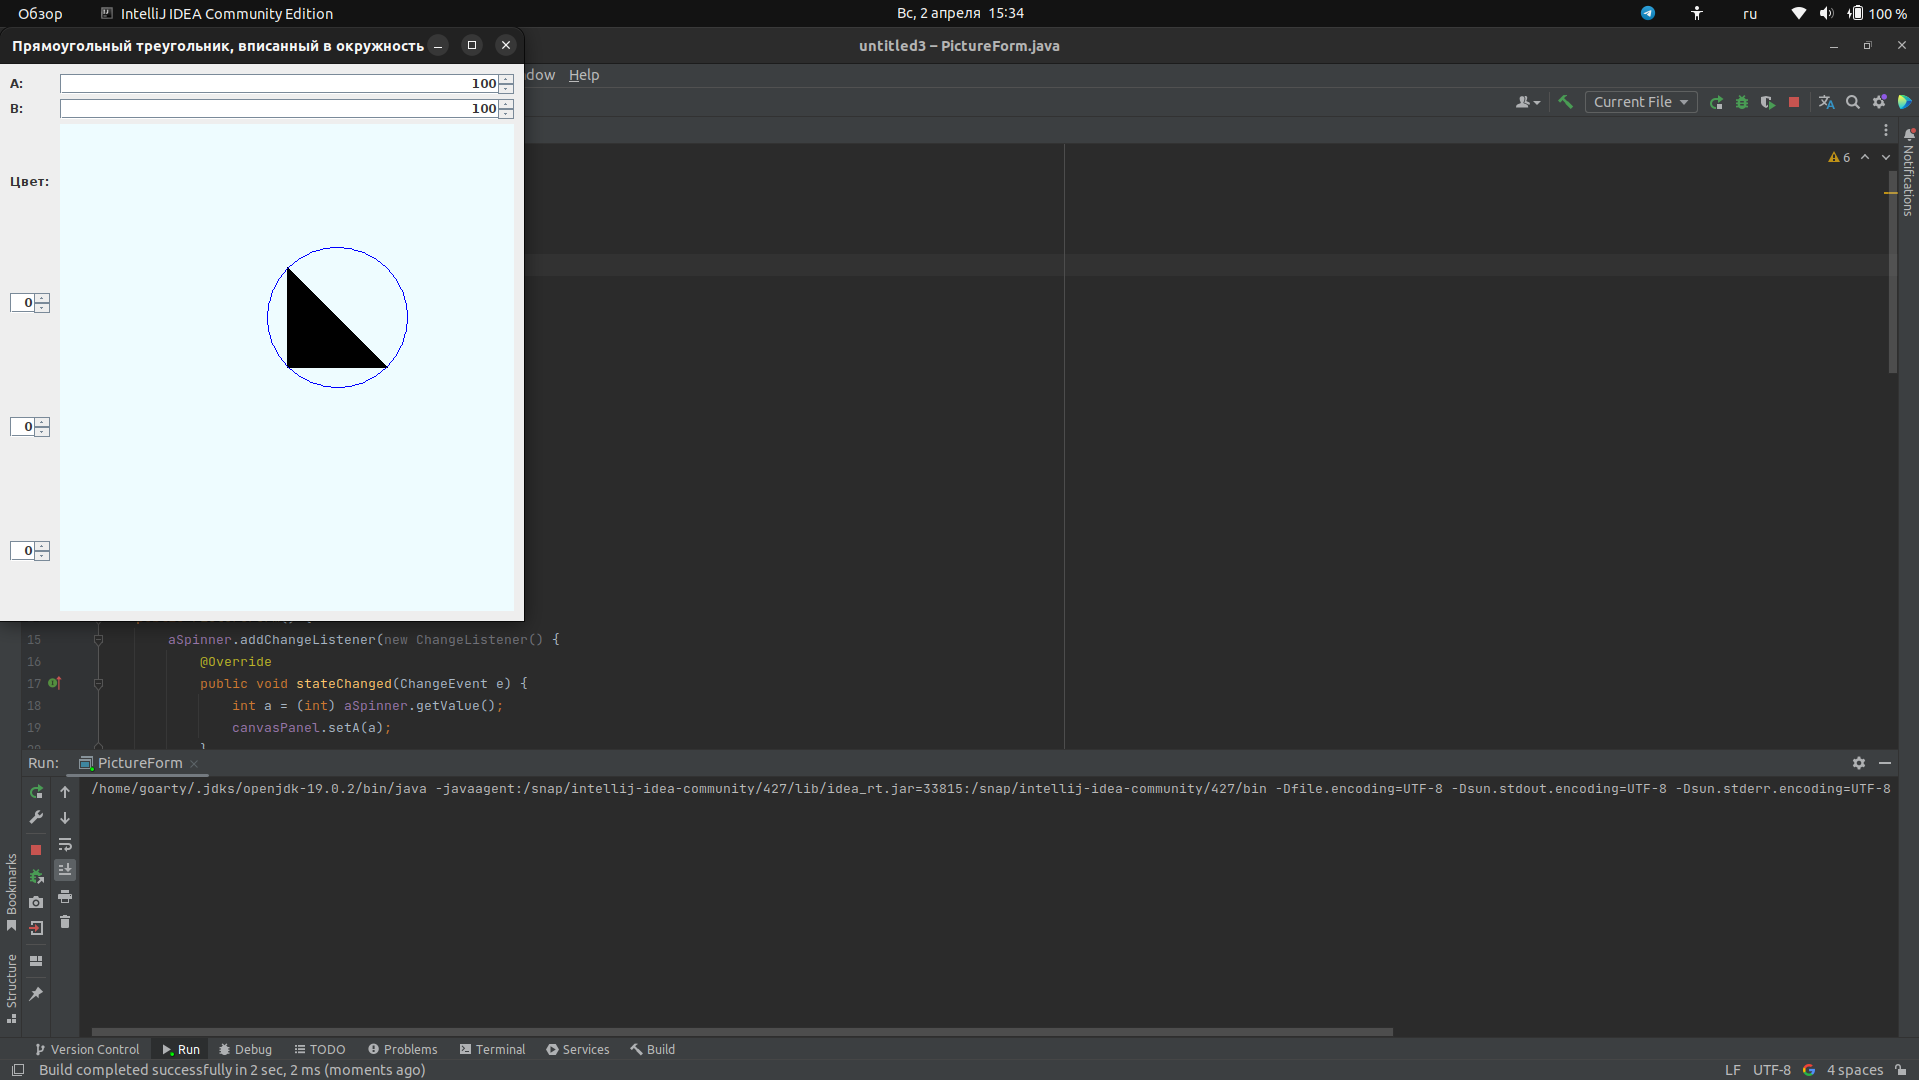
\includegraphics[width=0.8\textwidth]{picture_1.png}
\caption{Реализация main.cpp}
\label{fig:picture_1.png}
\end{figure}

\begin{figure}[!htb]
	\centering
	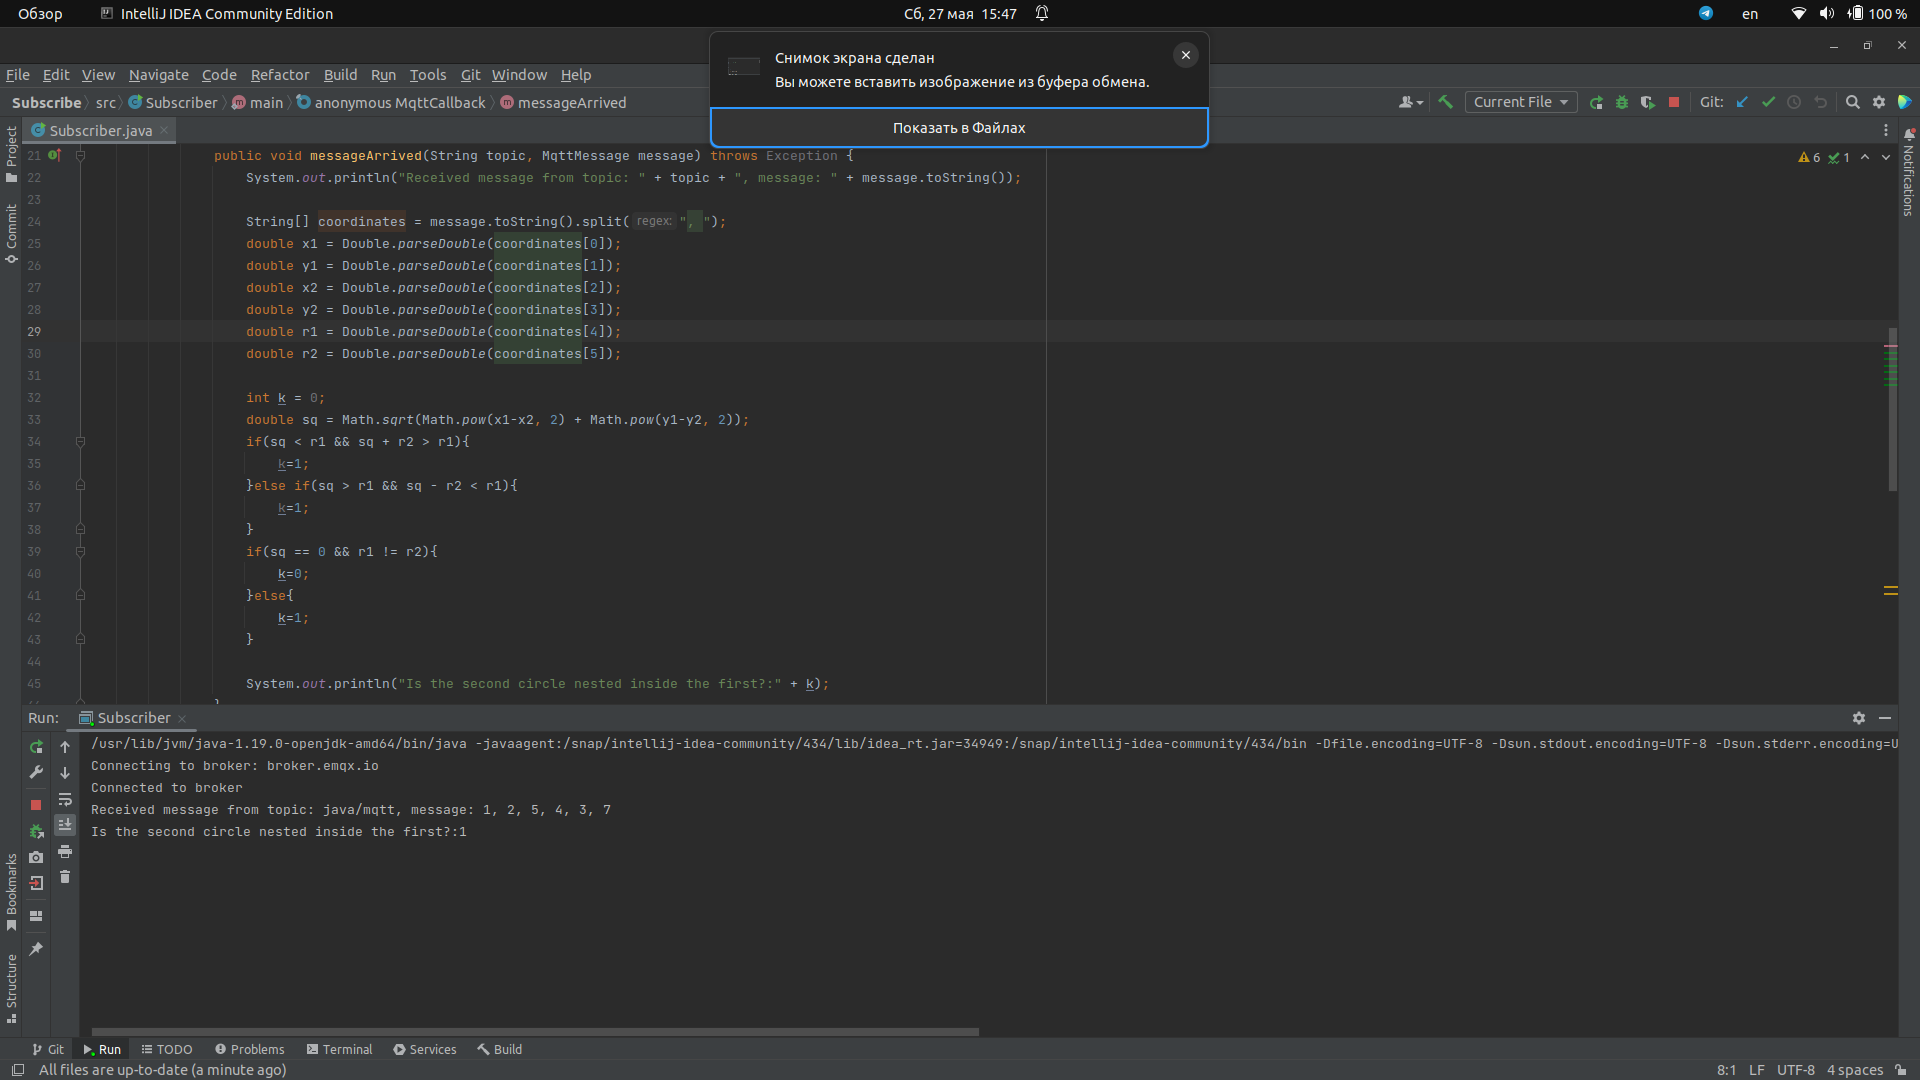
\includegraphics[width=0.8\textwidth]{picture_2.png}
\caption{Реализация и Set.h}
\label{fig:picture_2.png}
\end{figure}

\begin{figure}[!htb]
	\centering
	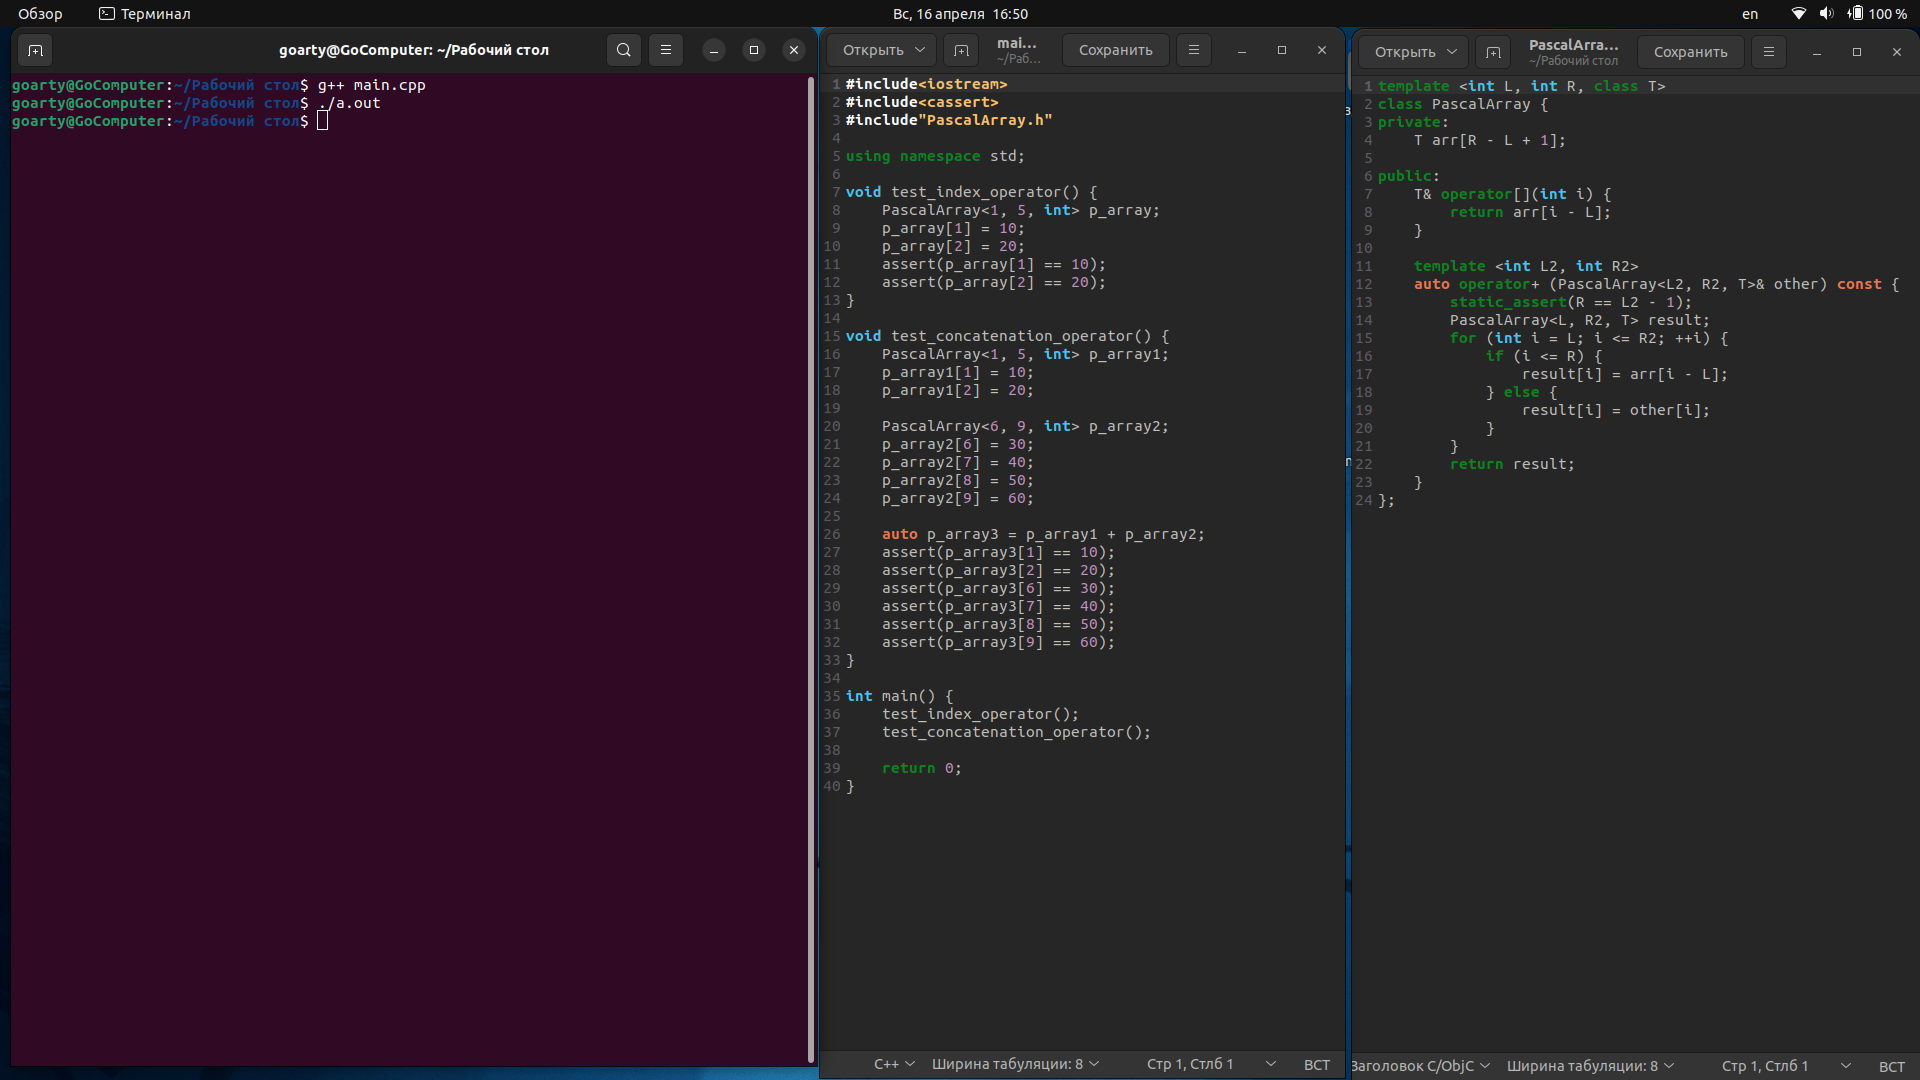
\includegraphics[width=0.8\textwidth]{picture_3.png}
\caption{Работа программы}
\label{fig:picture_3.png}
\end{figure}

\end{document}
